\section{RENI++: A Statistical Model of Natural Illumination}\label{sec:RENI}

We now describe how to construct a statistical model of natural illumination environments as a rotation-equivariant conditional spherical neural field trained on a dataset of HDR outdoor illuminations. Natural environments have a canonical ''up'' direction (defined by gravity) but arbitrary rotation about this vertical axis. For this reason, in our model of natural illumination we do not want full $SO(3)$ rotation equivariance. This would have the undesirable effect of permitting unnatural environment orientations (such as with the sky at the bottom), providing a less useful prior when solving inverse problems. We therefore use the $SO(2)$ invariant formulation in Section \ref{sec:SO2} with the equivariant rotation axis set to the vertical ($y$) axis: $\mathbf{a}=\mathbf{e}_y$. This means that our model is also equivariant to reflections about planes parallel to the up direction. This is also a useful property. For example, consider an environment with the sun to the right of a tree. Our model could represent with the same accuracy (and via a reflection of the latent code) a reflected version of the environment with the sun to the left of a tree. This ability to represent any rotation or reflection of an environment without the need for any rotation or reflection augmentation.

We named our original model RENI (Rotation-Equivariant Natural Illumination) \cite{gardner2022rotation}. Here, we name our extended model RENI++ and explain below our new scale-invariant property, HDR representation, underlying neural field architecture and the training data and losses used in our implementation.

\subsection{Training Data} 
\label{Training Data}
HDR illumination is essential for realistic rendering and enables the accurate representation of the full dynamic range of natural light. Therefore our model must learn an HDR representation of natural illumination. We have curated a dataset of HDR equirectangular images of outdoor, natural illumination environments obtained with a CC0 1.0 Universal Public Domain Dedication license \cite{poly_haven_hdris_nodate, giantcowfilms_hdris_nodate, ihdri_hdris_nodate, hdrmaps_hdris_nodate, whitemagus_3d_hdris_nodate, hdri_skies_hdris_nodate, textures_hdris_nodate}. All images were then checked to ensure they did not contain any personally identifiable information or offensive content and any images that contained predominantly unnatural light sources were removed. $21$ images were also selected and held back for optimising only the latent codes at test time, resulting in a training dataset of 1,673 HDR images.

Each training batch comprises $P$ pairs of directions and corresponding log scaled $\text{log}(\text{HDR})$ RGB colours that we store in the matrices $\mathbf{D}=[\mathbf{d}_{1},\dots,\mathbf{d}_{P}]\in\R^{3\times P}$ and $\mathbf{C}=[\mathbf{c}_{1},\dots,\mathbf{c}_{P}]\in\R^{3\times P}$ respectively. Each batch contains samples distributed across all the images in the training set. As RENI++ is a continuous neural field, it is agnostic to the resolution and sampling of the spherical signal. The neural field can be queried for any direction. In practice, our dataset contains equirectangular spherical images. Because equirectangular images feature irregular sampling, we select directions according to the following criteria:
\begin{itemize}
    \item For the azimuthal angle \( \theta \), we sample uniformly in the interval \( [0, 2\pi] \):
\[
\theta \sim \mathcal{U}(0, 2\pi)
\]
\item For the polar angle \( \phi \), we sample according to a probability density function \( g(\phi) \) defined on \( [0, \pi] \):
\[
g(\phi) = \frac{\sin(\phi)}{2}
\]
Here, the division by 2 normalizes \( g(\phi) \) to ensure its integral is equal to 1.
\item Finally we round these samples down to the nearest discrete pixel location.
\end{itemize}
In contrast to RENI \cite{gardner2022rotation}, in which each batch contained all rays from a single image and a sine-weighting in the loss function was used to compensate for the irregular sampling, we empirically found this new sampling procedure smoothed the loss landscape and removed the requirement for multi-resolution training.

\subsection{High Dynamic Range Scale Invariance}
Computing a reconstruction loss in linear HDR space is dominated by large values and leads to a poor reconstruction of most of the environment. Therefore, similar to \cite{eilertsen_hdr_2017}, we train our network to output $\text{log}(\text{HDR})$ values and compute losses in log space. 

As the HDR images in our dataset are at unknown exposure values (EV) any image could be scaled by a global constant and would still represent a possible environment, simply one captured at a different EV. Therefore training RENI++ using an L2 reconstruction loss directly on pixel values, as was done in our prior work, results in over-fitting to the arbitrary EVs of images in the training data. This results in the latent space struggling to represent out-of-distribution EVs. To address this we take inspiration from monocular depth estimation techniques \cite{eigenDepthMapPrediction2014, liMegaDepthLearningSingleView2018} and train RENI++ using a scale-invariant loss:
\begin{equation}
  \mathcal{L}_{\text {scale-inv}}=\frac{1}{P} \sum_{p=1}^P\left(R_p\right)^2-\frac{1}{P^2}\left(\sum_{p=1}^P R_p\right)^2,
\end{equation}
where $R_{p} = f(\mathbf{d}_p^\prime, \mathbf{Z}^\prime_p) - \text{log}(\mathbf{c}_p)$ at pixel $p$ and $\mathbf{Z}^\prime_p$ is the invariant representation of the latent code of the image from which the $p$th pixel in the batch was drawn. This computes the mean square error (MSE) of the difference between all pairs of log-depths in linear time and results in the latent space of our model now representing a scale-free HDR image. Since the output of our model is only up to an unknown scale, we compute an optimal scale between reconstruction and ground truth before computing metrics. In practice, we do this using ordinary least squares in log space. We found that computing the optimal scale in linear space had no significant effect on the final metrics. In an inverse rendering setting, this scale becomes a per-image optimisable parameter representing the overall brightness of the environment.

To encourage accurate colour reproduction we also include a cosine similarity loss $\mathcal{L}_\text{cosine}$ on the RGB colour vectors:
\begin{equation}\label{cosine_similarity_loss}
    \mathcal{L}_{\text{cosine}} = 1.0 - \frac{1}{P} \sum_{i=1}^P \frac{f(\mathbf{d}_p^\prime, \mathbf{Z}^\prime_p) \cdot \text{log}(\mathbf{c}_p)}{\|f(\mathbf{d}_p^\prime, \mathbf{Z}^\prime_p)\| \|\text{log}(\mathbf{c}_p)\|}
\end{equation}

Since this only penalises the error in the RGB direction, it too is scale-invariant.

\subsection{Variational Auto-decoder}
We train our conditional spherical neural field as a decoder-only architecture, i.e. an auto-decoder \cite{park_deepsdf_2019} or Generative Latent Optimisation \cite{bojanowskiOptimizingLatentSpace2018}. This means that we optimise the network weights simultaneously with the latent codes for each training sample. This avoids the need to design a rotation-equivariant encoder while, for inverse tasks, only the decoder is needed so we avoid the redundancy of also training an encoder. However, training with no regularisation on the learnt latent space does not lead to a space that is smooth or that follows a known distribution. This means it cannot be sampled from, does not produce meaningful interpolations and provides no prior for inverse problems. For this reason, we use a \emph{variational auto-decoder} \cite{zadeh_variational_2021} architecture. Each training sample is represented by a mean, $\boldsymbol{\mu}_{i}\in\R^{3N}$, and standard deviation, $\boldsymbol{\sigma}_{i}\in\R^{3N}$, that provide the parameters of a normal distribution from which the flattened latent code for that training sample is drawn: $\text{vec}(\mathbf{Z}_i)\sim\mathcal{N}(\boldsymbol{\mu}_{i},\boldsymbol{\Sigma}_i)$, where $\boldsymbol{\Sigma}_i=\text{diag}(\sigma_{i,1}^2,\dots,\sigma_{i,3N}^2)$ is the diagonal covariance matrix. Using the reparameterisation trick \cite{kingma_auto-encoding_2013}, we can generate a latent code \(\text{vec}(\mathbf{Z}_{i}) = \boldsymbol{\mu}_{i}+ \boldsymbol{\sigma}_{i} \odot \boldsymbol{\epsilon}\) where the noise is sampled as \(\boldsymbol{\epsilon} \sim \mathcal{N}(\mathbf{0}, \mathbf{I}_{3N})\). During training, we optimise $\boldsymbol{\mu}_{i}$ and  $\boldsymbol{\sigma}_{i}$ for each training sample and use the Kullback–Leibler divergence (KLD) as a loss to regularise the distribution of each latent code toward the standard normal distribution:
\begin{equation}\label{kld_loss}
    \mathcal{L}_{\text{KLD}}= -\frac{1}{2}\sum_{i=1}^{K}\frac{1}{D}\sum_{j=1}^{D}(1 + \log(\sigma_{i,j}^{2})-\mu_{i,j}^{2} - \sigma_{i,j}^{2}),
\end{equation}
where $K$ is the number of unique latent codes in a batch, and $D = 3N$ is the dimensionality of the latent space.

\subsection{Neural Field} 
Our neural field decoder, $f$, is conditioned using cross-attention layers as per \cite{rebainAttentionBeatsConcatenation2023}. Similar to the Transformer decoder \cite{vaswaniAttentionAllYou2017} architecture, our neural field operates as follows.

For each layer \( l \) in the decoder, we apply multi-head attention (MHA):
\begin{equation}
    \text{MHA}^l(\mathbf{Q}, \mathbf{K}, \mathbf{V}) = \text{Concat}(\text{head}_1^l, \ldots, \text{head}_h^l)W^O + \mathbf{Q},
\end{equation}
and a position-wise feed-forward network (FFN):
\begin{multline}
\text{FFN}^l(\mathbf{d}'^{(l-1)}) = \text{LN}(\mathbf{d}'^{(l-1)}) \\
\quad + \text{ReLU}(\text{LN}(\mathbf{d}'^{(l-1)})W_1^l + b_1^l)W_2^l + b_2^l,
\end{multline}
where $ \mathbf{Q} = \mathbf{d}^\prime W^Q $, $ \mathbf{K} = \mathbf{Z}^\prime W^K $, and $ \mathbf{V} = \mathbf{Z}^\prime W^V $ and $\text{LN}$ is the layer norm operation. Here, $ \mathbf{d}^\prime $ is the output from the previous layer or the original input for the first layer, $ \mathbf{Z}^\prime $ is the conditioning input, and the heads correspond to different projections of these inputs. Residual connections are applied around both the MHA and FFN modules, with layer normalisation following each residual connection.

The output of the final layer $L$ is then passed through an output projection to predict HDR RGB values:
\begin{equation}
\text{Output} = \sigma(\text{FFN}^L(\mathbf{d}'^L)W^{\text{out}} + b^{\text{out}}).
\end{equation}
An optional non-linearity $ \sigma $ activation function is applied at the output stage.

The original RENI model \cite{gardner2022rotation} used \emph{conditioning-by-concatenation} \cite{sitzmann_implicit_2020, xie_neural_2021}, i.e.~both the directional, $\mathbf{d}^\prime$, and conditioning, $\mathbf{Z}^\prime$, inputs were passed directly as input to the first layer of the decoder network. This decoder network was a SIREN \cite{sitzmann_implicit_2020}, an MLP with a periodic activation function, as this architecture had proven highly effective at representing a wide range of complex natural signals. However similar to \cite{rebainAttentionBeatsConcatenation2023} we found attention with positional encoding on directions outperformed the \emph{conditioning-by-concatenation} SIREN and \cite{sitzmann_implicit_2020, xie_neural_2021} and \emph{FiLM-conditioned} \cite{chan_pi-gan_2021} SIREN when fitting latent codes to unseen images.


\begin{figure}
    \centering
    \makebox[\columnwidth]{%
        \begin{tikzpicture}
        % \draw[step=0.5cm,gray,very thin] (-3,-2) grid (3,2);
        \node (img) {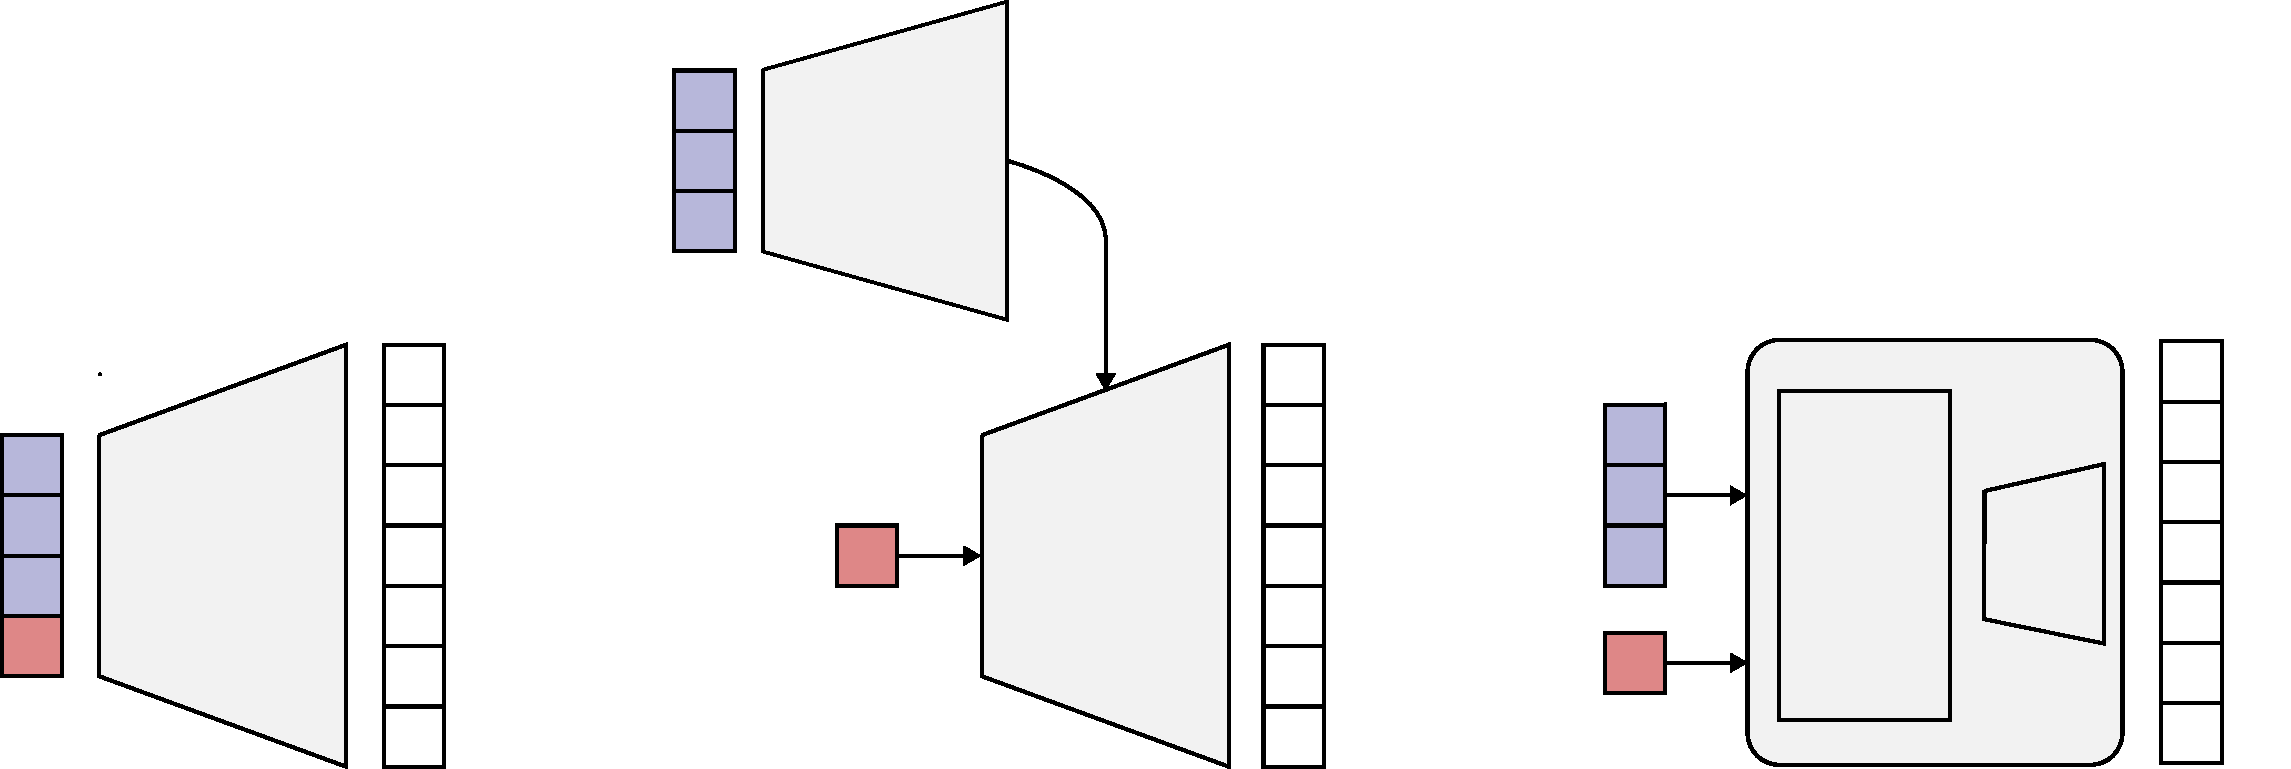
\includegraphics[width=0.90\columnwidth]{Figures/model_types.pdf}};
    
        % Add 'outputs' labels rotated by 90 degrees
        \node[rotate=90, font=\tiny] at (-2.29, -0.60) {outputs};
        \node[rotate=90, font=\tiny] at (0.76, -0.60) {outputs};
        \node[rotate=90, font=\tiny] at (3.9, -0.60) {outputs};
    
        % Add 'z' labels for the orange inputs
        \node[font=\tiny] at (-4.15, -0.48) {z};
        \node[font=\tiny] at (-1.79, 0.8) {z};
        \node[font=\tiny] at (1.45, -0.38) {z};
    
        % Add 'λ(x)' labels for the red inputs
        \node[font=\tiny] at (-4.3, -0.92) {$\lambda(d)$};
        \node[font=\tiny] at (-1.38, -0.59) {$\lambda(d)$};
        \node[font=\tiny] at (1.3, -0.97) {$\lambda(d)$};
    
        % Add 'MLP' in each of the networks
        \node[font=\tiny] at (-3.2, -0.59) {MLP};
        \node[font=\tiny] at (-0.1, -0.59) {MLP};
        \node[rotate=90, font=\tiny] at (3.15, -0.59) {MLP};
    
        % Add 'MLP' in each of the networks
        \node[font=\tiny] at (-3.2, -1.7) {Condition-by-Concat};
        \node[font=\tiny] at (0.0, -1.7) {Hypernetwork};
        \node[font=\tiny] at (2.8, -1.7) {Attention};
    
        % Extra
        \node[font=\tiny] at (-0.85, 0.95) {Hyper};
        \node[font=\tiny] at (-0.85, 0.65) {MLP};
        \node[font=\tiny] at (-0.0, 0.75) {\textbf{W}};
        \node[font=\tiny] at (2.35, -0.24) {K};
        \node[font=\tiny] at (2.35, -0.50) {V};
        \node[font=\tiny] at (2.35, -0.97) {Q};
    
        \end{tikzpicture}
    }
    \caption{Three methods of conditioning in Neural Fields. Similar to \cite{rebainAttentionBeatsConcatenation2023} we found \emph{attention} outperformed \emph{conditioning-by-concatenation} and \emph{FiLM-conditioning} in capturing high-frequency details. $\lambda$ is a positional encoding \cite{mildenhall_nerf_2020} applied to the inputs.}
    \label{fig:model_types}  
\end{figure}

\subsection{Training} \label{Training Details}
RENI++ is implemented in Nerfstudio \cite{nerfstudio}, a framework for developing Neural Field based applications. We use Adam \cite{kingma_adam_2015}, along with a Cosine Decay \cite{loshchilov2017sgdr} schedule and 500-step 'warm-up' phase, to optimise the sum of the scale-invariant and KLD losses:
\begin{equation}\label{training_loss}
    \mathcal{L}_{\text{Train}} = \rho \mathcal{L}_{\text{scale-inv}} + \gamma \mathcal{L}_{\text{cosine}} + \beta \mathcal{L}_{\text{KLD}}
\end{equation}
We randomly initialise the mean latent code for each image, \(\boldsymbol{\mu}_{i}\), from a standard normal distribution. In order to ensure the positivity of the variances, $\sigma^2_{i,j}$, we optimise $\log(\sigma^2_{i,j})$ which we initialise randomly from a normal distribution with mean -5 and variance 1. With the new sampling procedure and model architecture described above we found better performance than the conference paper even when training for $80x$ fewer steps. We found the best performance when using a transformer-based variational auto-decoder with $8$ attention heads $6$ decoder layers and $128$ parameters per layer. We use a cosine decaying learning rate \cite{loshchilov2017sgdr} with a warm-up phase modelled as:

$$\text{lr} = \text{lr}_{0} \times \frac{s}{\text{W}}$$

Where $W$ is the number of warm-up steps, $\text{lr}_{0}$ is the initial learning rate and $s$ is the current step. The post-warm-up learning rate is then computed via:

$$\text{lr} = \text{lr}_{0} \times \left( \alpha + \frac{1 - \alpha}{2} \times (\cos(\pi \times \frac{s - \text{W}}{s_{\text{max}} - \text{W}}) + 1) \right) $$

Where $s_\text{max}$ is the maximum number of training steps and $\alpha$ is the minimum learning rate as a fraction of the initial learning rate. We use a $500$-step warm-up phase, $\alpha = 5 \times 10^{-2}$ and an initial learning rate of \(10^{-3}\). Our loss weights are \(\rho=1.0\), \(\gamma=1.0\) and \(\beta=10^{-6}\). Training RENI++ with a latent code dimension of $D = 27$, $\text{num heads} = 8$, $\text{num layers} = 6$, $\text{hidden features} = 128$ and NeRF \cite{mildenhall_nerf_2020} positional encoding on the directions takes around 15 minutes on an Nvidia RTX 3080-Ti 16GB Laptop GPU.

\subsection{Model Fitting} At test time the decoder is held static and only latent codes are optimised to fit an unseen image. We initialise the latent code to zeros, corresponding to the mean environment map (see Figure \ref{fig:teaser}, left). This provides an unbiased initialisation in the absence of any prior information about the environment. We use the same losses as used during training except we remove $\mathcal{L}_{\text{KLD}}$. Our test time loss is therefore:
\begin{equation}\label{test_loss}
    \mathcal{L}_{\text{Test}} = \rho \mathcal{L}_{\text{scale-inv}} + \gamma \mathcal{L}_{\text{Cosine}}
\end{equation}
We found the best performance when using $\rho = 1.0$, $\gamma = 1.0$, and Adam with an exponentially decaying learning rate starting at \(10^{-1}\) and decreasing to \(10^{-7}\) over $2500$ steps. This takes around $1$ minute to fit all $21$ images in the test dataset on an Nvidia RTX 3080-Ti 16GB Laptop GPU.

A PyTorch implementation, our dataset and trained models can be found at \href{https://github.com/JADGardner/ns_reni}{github.com/JADGardner/ns\_reni}.
